\section{Hard Families for Graph Neural Networks}\label{sec:HardFamilies}



\subsection{Family $\{(\GraphG_\ess^\kay,\, \GraphH_\ess^\kay)\}_{\ess \in \N}$}

In this section, we introduce the family of graph pairs $\Fam_\kay = \{(\GraphG_\ess^\kay,\GraphH_\ess^\kay)\}_{\ess \in \N}$ and establish its relevant properties. We start with graph class $\{\GraphG_\ess^\kay\}_{\ess \in \N}$ whose pairing with $\{\GraphH_\ess^\kay\}_{\ess \in \N}$ forms class $\Fam_\kay$.

We let graph $\GraphG_0^\kay = \CompleteGraph_\kay \square \Cycle_2$ be the cartesian product of the complete graph on $\kay$ vertices, and the 2-cycle $\Cycle_2$. This consists of two disjoint $\CompleteGraph_\kay$ subgraphs and a perfect matching of edges between vertices of each $\CompleteGraph_\kay$ subgraph (see figure \ref{fig:G[3,1]}). 

\begin{figure}[h]
    \centering
    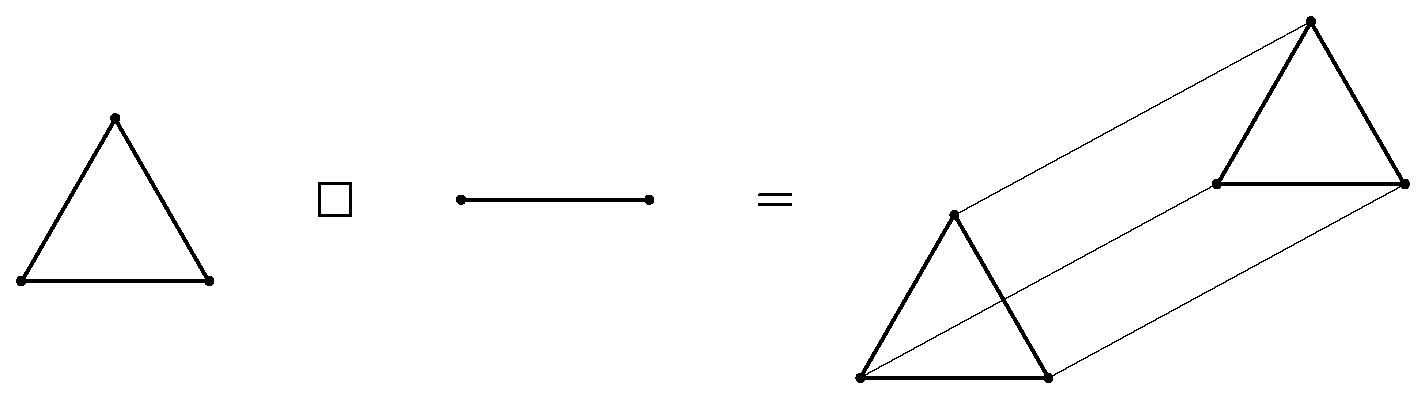
\includegraphics[width=0.5\linewidth]{ICML 2026/Figures/G[3,1].eps}
    \caption{Graph $\GraphG_0^3$}
    \label{fig:G[3,1]}
\end{figure}

Graph  $\GraphG_0^\kay$ can equivalently be defined as $(\CompleteGraph_\kay \square \Cycle_2) \square \Cycle_0$.\footnote{We take $\Cycle_0$ to be a single vertex with no edges.} By consecutively taking products of $\GraphG_0^\kay$ with $\Cycle_\enn$ for each $\enn \in 2\N$, we straightforwardly obtain the family $\{\GraphG_s^\kay\}_{s \in \N}$:\footnote{For convenience in the proofs, we take graph products only with even cycles, whose chromatic number is~2.}
$$\GraphG_s^\kay = (\CompleteGraph_\kay \square \Cycle_2) \square \Cycle_{s\cdot 2}.$$

Next we define graph class $\{\GraphH_\ess^\kay\}_{\ess \in \N}$. At the base of this graph class will be a modification of graph $\GraphG_0^\kay$ which we term a "\emph{rewiring}" of $\GraphG_0^\kay$. 

Let graph $\GraphG = \CompleteGraph_\kay \square \Cycle_2$ with vertex set $\VertexSet(\GraphG) = \{\vertexv_0, \ldots, \vertexv_{2\kay-1}\}$ where vertices $\VertexSet_{K'}=\{\vertexv_0, \ldots, \vertexv_{\kay-1}\}$ and vertices $\VertexSet_{K''}=\{\vertexv_\kay, \ldots, \vertexv_{2\kay-1}\}$ respectively make up the vertices of each disjoint $\CompleteGraph_\kay$ subgraph, $K'$ and $K''$, of $\GraphG$. Moreover, let edge set $\EdgeSet_m = \{(\vertexv_i,\vertexv_{i+\kay}): i \in \dbset{\kay}\}$ be the subset of $\EdgeSet(\GraphG)$ consisting of the perfect matching between vertices in $\VertexSet_{K'}$ and vertices in $\VertexSet_{K''}$. We let $\GraphH_0^\kay$ be the graph with vertex set $\VertexSet(\GraphH) = \VertexSet(\GraphG)$ and edge set $\EdgeSet(\GraphH)$ equal to,
$$[\EdgeSet(\GraphG)\setminus\{(\vertexv_i,\vertexv_j),(\vertexv_{i+k},\vertexv_{j+k})\}] \cup \{(\vertexv_i,\vertexv_{j+k}),(\vertexv_{i+k},\vertexv_{j})\}$$
for exactly one $i \in \dbset{\kay}$ and one $j \in \dbset{\kay}$ ($j\neq i$). Intuitively, graph $\GraphD_0^\kay$ is the modification of $\GraphG_0^\kay$ where for exactly one edge $(\vertexv_i,\vertexv_j)$ of clique subgraph $K'$, its endpoint $\vertexv_j$ is changed to $\vertexv_{j+k}$ and for corresponding edge $(\vertexv_{i+k},\vertexv_{j+\kay})$ of clique subgraph $K''$ endpoint $\vertexv_{j+k}$ is changed to $\vertexv_{j}$.


\begin{figure}[h]
    \centering
    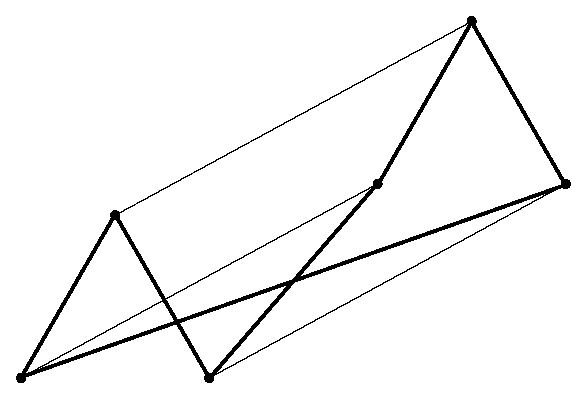
\includegraphics[width=0.5\linewidth]{ICML 2026/Figures/H[3,1].eps}
    \caption{Graph $\GraphH_0^3$}
    \label{fig:H[3,1]}
\end{figure}

Having defined $\GraphH_0^\kay$ we again consecutively take products of $\GraphH_0^\kay$ with $\Cycle_\enn$ for each $\enn \in 2\N$ and straightforwardly obtain family $\{\GraphH_\ess^\kay\}_{\ess \in \N}$. 
$$\GraphH_s^\kay = \GraphH_0^\kay \square \Cycle_{s\cdot 2}$$

The next proposition summarizes relevant properties of family $\{(\GraphG_\ess^\kay,\, \GraphH_\ess^\kay)\}_{\ess \in \N}$. (We defer all proofs in section \ref{sec:HardFamilies} to Appendix \ref{app:HardFamilies}).
\begin{proposition}\label{prop:GraphClassGProps}
    For any  $\kay \geq 3$ and any $\ess \in \N$ family $\{(\GraphG_\ess^\kay,\, \GraphH_\ess^\kay)\}_{\ess \in \N}$, satisfies the following properties.
    \begin{enumerate}
        \item $|\VertexSet(\GraphG_\ess^\kay)|= |\VertexSet(\GraphH_\ess^\kay)|$ \label{GraphClassGPropsVertexNum}
        %$|\VertexSet(\GraphG_\ess^\kay)|= |\VertexSet(\GraphH_\ess^\kay)| = 2\kay \cdot (\ess + 1)$
        \item $\reg(\GraphG_\ess^\kay)=\reg(\GraphH_\ess^\kay)$\label{GraphClassGPropsRegularity}
        %$\reg(\GraphG_\ess^\kay)=\reg(\GraphG_\ess^\kay)=3\cdot(\kay +1)$, for $\ess \geq 2$
        \item $\omega(\GraphG_\ess^\kay) = \kay$ \label{GraphClassGPropsCliqueNum}
        \item $\chi(\GraphH_\ess^\kay) = \kay-1$ \label{GraphClassGPropsChromaticNum}
    \end{enumerate}
\end{proposition}
% \begin{proof}
%      \textbf{\ref{GraphClassGPropsVertexNum}.}
%      Graph $\GraphG_0^\kay$ and its rewiring $\GraphG_0^\kay$ have the same number of vertices since no vertices are added or subtracted under rewiring. Any product of each of these graphs with a cycle $\Cycle_\enn$ preserves this equality.
    
%     \textbf{\ref{GraphClassGPropsRegularity}.}
%     Let graph vertex sets $\VertexSet_{K'}=\{\vertexv_0, \ldots, \vertexv_{\kay-1}\}$ and $\VertexSet_{K''}=\{\vertexv_\kay, \ldots, \vertexv_{2\kay-1}\}$ respectivley make up the vertices of each disjoint $\CompleteGraph_\kay$ subgraph, $K'$ and $K''$, of $\GraphG_0^\kay$.
%     Under rewiring of $\GraphG_0^\kay$, for exactly one edge $(\vertexv_i,\vertexv_j)$ of clique subgraph $K'$, its endpoint $\vertexv_j$ is changed to $\vertexv_{j+k}$ and for corresponding edge $(\vertexv_{i+k},\vertexv_{j+1})$ of clique subgraph $K''$ endpoint $\vertexv_{j+k}$ is changed to $\vertexv_{j}$. In this process $\vertexv_j$ loses and gains one neighbor, so regularity is preserved and equality $\reg(\GraphG_0^\kay)=\reg(\GraphG_0^\kay)$ holds. Any product of each of these graphs with a cycle $\Cycle_\enn$ preserves this equality by point \ref{GraphProdReg} of Proposition \ref{prop:SabidussiCombinedGeneral}.
    
%     \textbf{\ref{GraphClassGPropsCliqueNum}.} 
%     Since each $\GraphG_\ess^\kay$ is the product of $\CompleteGraph_\kay$ and two cycles, point \ref{GraphClassGPropsCliqueNum} follows from point \ref{ProdCliqInvsKC} of Proposition \ref{obs:ProdCliqInvs}.

%     \textbf{\ref{GraphClassGPropsChromaticNum}.}
%     We assume without loss of generality that edges $(\vertexv_0, \vertexv_1)$ and $(\vertexv_\kay, \vertexv_{\kay+1})$ of $\GraphG_0^\kay$ are rewired under $\GraphG_0^\kay$. Let coloring $\coloring: \VertexSet(\GraphG_0^\kay) \rightarrow \dbset{\kay-1}$ be defined such that $\coloring(\vertexv_0) = \coloring(\vertexv_1) = 0$ and $\coloring(\vertexv_i) = i-1$ for $i \in \{2, \ldots, \kay-1\}$. This coloring properly colors vertices in $\VertexSet_{K'}$ since vertices, $\vertexv_0$ and $\vertexv_1$ are non adjacent in $\GraphG_0^\kay$. We now extend coloring $\coloring$ to assign colors $\coloring(\vertexv_{\kay}) = \coloring(\vertexv_{\kay+1}) = \kay-2$ and $\coloring(\vertexv_{\kay + i}) = i-2$ for $i \in \{2, \ldots, \kay-1\}$. The colors of vertices $\vertexv_0,\vertexv_1$ do not conflict with their neighbors $\vertexv_{\kay+1},\vertexv_{\kay + i}$ in $\VertexSet_{K''}$ since $\coloring(\vertexv_0) = \coloring(\vertexv_1) = 0 \neq \kay-2 =\coloring(\vertexv_{\kay}) = \coloring(\vertexv_{\kay+1})$. More generally, for $i \in \{2, \ldots, \kay-1\}$ vertex $\vertexv_i$ does not conflict with its neighbor $\vertexv_{\kay+i}$ since $\coloring(\vertexv_i) = i-1\neq i-2 = \coloring(\vertexv_{\kay + i})$.
% \end{proof}

The properties of Proposition \ref{prop:GraphClassGProps} together with Observation \ref{obs:WL-regular-undistinguished} and Proposition \ref{prop:GNN-iff-WL} immediately imply the following theorem.

\begin{theorem}\label{thm:Ind1GNN}
    Let $\mathcal{N}$ be a message-passing graph neural network. Then for any pair of graphs $(\GraphG, \GraphH)$ of family  $\{(\GraphG_\ess^\kay,\, \GraphH_\ess^\kay)\}_{\ess \in \N}$, $\GNN(\GraphG) = \GNN(\GraphH)$.
\end{theorem}
% \begin{proof}
%     By Proposition \ref{prop:GraphClassGProps} graphs $\GraphG$ and $\GraphH$ are an the same number of vertices and have the same regularity. Hence, $\GNN(\GraphG) = \GNN(\GraphH)$ by Observation \ref{obs:WL-regular-undistinguished} and Proposition \ref{prop:GNN-iff-WL}.
% \end{proof}


\subsection{Indistinguishable for 2-WL. Easy for 3-WL.}

With only minor additional technical arguments, one can show that the family $\Fam_\kay$ is also indistinguishable by $2$-WL, and hence by $2$-GNNs.

\begin{theorem}\label{thm:Ind2-GNN}
    Let $\mathcal{N}_2$ be a 2-GNN. Then for any pair $(\GraphG,\GraphH)$ in the family
    $\{(\GraphG_\ess^\kay,\, \GraphH_\ess^\kay)\}_{\ess \in \N}$, we have $\mathcal{N}_2(\GraphG)=\mathcal{N}_2(\GraphH)$.
\end{theorem}

The above result is consistent with the known expressivity relationship between 1‑WL and 2‑WL. Under the "non-folklore" refinement definition, the two methods are equivalent for isomorphism testing \citep{inproceedings}.
% \begin{proof}
%     We show that 2-WL stabilizes in two steps. That is, we show that for any pair $(\GraphG,\GraphH)$ in $\{(\GraphG_\ess^\kay,\, \GraphH_\ess^\kay)\}_{\ess \in \Nplus}$, the cardinalities of initial coloring $\coloring^{(0)}$ and consecutive coloring $\coloring^{(1)}$ are equal. 

%     Without loss of generality we assume that initial coloring $\coloring^{(0)}$ assigns to each edge color $\coloring_1$ and each non-edge color $\coloring_2$ where $\coloring_1 \neq \coloring_2$. By points \ref{GraphClassGPropsVertexNum} and \ref{GraphClassGPropsRegularity} of \ref{prop:GraphClassGProps} graphs $\GraphG$ and $\GraphH$ have the same number of edges and non-edges. Let $\edgee$ and $\nonedgee$ respectively be an edge and non-edge of $\EdgeSet(\GraphG) \cup \EdgeSet(\GraphH)$. We show that coloring $\coloring^{(1)}$ assigns color $\coloring_3$ to each edge $\edgee$ and $\coloring_4$ to each non-edge $\nonedgee$, where $\coloring_3 \neq \coloring_4$.

%     Let edge $\edgee = (\vertexu, \vertexv)$ be chosen arbitrarily from $\EdgeSet(\GraphG) \cup \EdgeSet(\GraphH)$. The set of neighbors of $\edgee$ is exactly the union of edges of $\GraphG$ ($\GraphH$) and non-edges of of $\GraphG$ ($\GraphH$) with one endpoint in $\edgee$ and one endpoint outside of $\edgee$. The number of edges incident to endpoint $\vertexu$ ($\vertexv$) is therefore given by $\reg-1$ (we do not count $\edgee$ itself) where $\reg$ is the regularity of $\GraphG$ ($\GraphH$)(recall that $\GraphG$ and $\GraphH$ have the same regularity of point \ref{GraphClassGPropsRegularity} of \ref{prop:GraphClassGProps}). Meanwhile, the number of non-edges incident to $\vertexu$ ($\vertexv$) is given by $|\VertexSet(\GraphG)| - \reg$ ($|\VertexSet(\GraphH)| - \reg$) (recall that vertex sets $\VertexSet(\GraphG)$ and $\VertexSet(\GraphH)$ have the same cardinality by \ref{GraphClassGPropsVertexNum} of \ref{prop:GraphClassGProps}). Hence and arbitrarily chosen $\edgee$ of $\EdgeSet(\GraphG) \cup \EdgeSet(\GraphH)$ has the same neighborhood and is assigned the same color under $\coloring^{(1)}$.

%     An analogous argument holds for arbitrarily chosen non-edges $\nonedgee$ of $\EdgeSet(\GraphG) \cup \EdgeSet(\GraphH)$.

%     Since color assignments under $\coloring^{1}$ are completely determined by isomorphism type, the image of $\coloring^{1}$ has the same cardinality as the image of $\coloring^{0}$.

    
% \end{proof}
% \begin{proof}
% We show that the $2$-WL refinement stabilizes after one refinement step. That is, for any pair
% $(\GraphG,\GraphH)$ in the family
% $\{(\GraphG_\ess^\kay,\, \GraphH_\ess^\kay)\}_{\ess \in \Nplus}$,
% the images of the initial coloring $\coloring^{(0)}$ and the refined coloring
% $\coloring^{(1)}$ have the same cardinality.

% Without loss of generality, assume that the initial coloring $\coloring^{(0)}$ assigns a color
% $\coloring_1$ to each edge and a distinct color $\coloring_2 \neq \coloring_1$ to each non-edge.
% By points~\ref{GraphClassGPropsVertexNum} and~\ref{GraphClassGPropsRegularity} of
% Proposition~\ref{prop:GraphClassGProps}, the graphs $\GraphG$ and $\GraphH$ have the same number
% of vertices, the same regularity, and consequently the same number of edges and non-edges.

% Let $\edgee = (\vertexu,\vertexv)$ be an arbitrary edge in
% $\EdgeSet(\GraphG) \cup \EdgeSet(\GraphH)$. In the $2$-WL refinement, the neighbors of $\edgee$
% are precisely the $2$-sets that share exactly one vertex with $\edgee$. These consist of all edges
% and non-edges incident to either $\vertexu$ or $\vertexv$, excluding $\edgee$ itself.

% Since both $\GraphG$ and $\GraphH$ are $\reg$-regular, each endpoint $\vertexu$ and $\vertexv$
% is incident to exactly $\reg - 1$ further edges. Moreover, as both graphs have the same number of
% vertices, the number of non-edges incident to each endpoint is
% $|\VertexSet(\GraphG)| - \reg$ (and likewise for $\GraphH$).
% Thus, every edge in $\EdgeSet(\GraphG) \cup \EdgeSet(\GraphH)$ has an identical multiset of
% neighbor colors under $\coloring^{(0)}$, and is therefore assigned the same color, say
% $\coloring_3$, under $\coloring^{(1)}$.

% An analogous argument applies to any non-edge
% $\nonedgee \in \EdgeSet(\GraphG) \cup \EdgeSet(\GraphH)$, showing that all non-edges receive a
% common color $\coloring_4 \neq \coloring_3$ under $\coloring^{(1)}$.

% It follows that the refined coloring $\coloring^{(1)}$ distinguishes edges from non-edges but
% introduces no further refinement. Hence, the image of $\coloring^{(1)}$ has the same cardinality
% as the image of $\coloring^{(0)}$, and the $2$-WL refinement stabilizes after one step.

% By Proposition~\ref{prop:kGNN-iff-kWL}, $2$-GNNs with injective aggregation and update functions
% cannot distinguish $\GraphG$ from $\GraphH$, and therefore
% $\mathcal{N}_2(\GraphG) = \mathcal{N}_2(\GraphH)$.
% \end{proof}

A straightforward triangle‑count argument on the base graphs 
$\{\GraphG_0^\kay\}$ and $\{\GraphH_0^\kay\}$ 
 shows that 3‑WL distinguishes our hard graph family in a single refinement round, and hence so does a suitably instantiated 3‑GNN by Proposition~\ref{prop:kGNN-iff-kWL}.


\begin{proposition}\label{prop:Dis3GNN}
Let $\mathcal{N}_3$ be a 3-GNN. There exist aggregation and update functions such that for any two graphs $\{\GraphG_0^\kay\}$ and $\{\GraphH_0^\kay\}$,
\[
\mathcal{N}(\GraphG_0^\kay) \neq \mathcal{N}(\GraphH_0^\kay),
\]    
for any $k \geq 3$.
\end{proposition}

Under experimental evaluation, we are able to specify a 3‑GNN that successfully distinguishes our hard graph family (see Appendix~\ref{app:Experiment3}).






































%\subsection{Generalization to dimension $d$}



